\pagebreak
\section{Motor Tests}
\nopagebreak
\subsection{Armature Resistance} %\label{put a label here and uncomment}
\textbf{Name: Group 510}\\
\textbf{Date: 30/09 - 2015}

\subsubsection{Purpose}
The purpose of the test is to measure the Armature resistance $R_a$.

\subsubsection{Setup}
\begin{figure}[H]
  \centering
	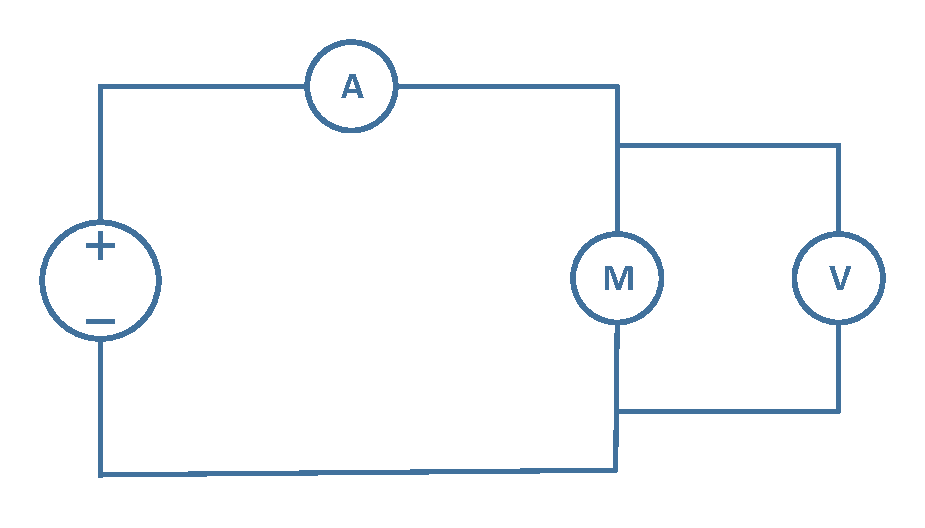
\includegraphics[scale=0.5]{figures/MotorTest1.pdf}
	\caption{Setup diagram}
\end{figure}

\subsubsection{List of Equipment}
Example of list of equipment:
\begin{table}[H]
\begin{tabular}{|l|l|p{4cm}|}
\hline%------------------------------------------------------------------------------------
  \textbf{Instrument}                        &  \textbf{AAU-no.}  &  \textbf{Type}       \\
\hline%------------------------------------------------------------------------------------
  Multimeter 1                               &  60764             &  Fluke 189 True RMS  \\
\hline%------------------------------------------------------------------------------------
  Multimeter 2                   		         &  60769             &  Fluke 189 True RMS  \\
\hline%------------------------------------------------------------------------------------
  Power Supply \small{(0 - 32 V) (0 - 10 A)} &  77076             &  Ea - ps 7032 - 100  \\
\hline%------------------------------------------------------------------------------------
  Clamp for fixing the motor                 &  03039             &                      \\
\hline%------------------------------------------------------------------------------------
\end{tabular}
\end{table}

\subsubsection{Procedure}

\begin{enumerate}
  \item Turn on the two multimeters and choose Voltage and Ampere setting respectively.
  \item Fix the motor shaft so it does not turn.
  \item Choose the first current value ($0.5$ A) on the current limiting of the power supply.
  \item Turn on the power supply and adjust the current limiting in accordance with the ampere meter.
  \item Repeat the two previous steps for each measurement of $0.5$ A increments up to $5$ A.
  \item Switch the poles of the power supply and repeat the measurements in the negative direction.
\end{enumerate}

\subsubsection{Results}

\begin{table}[H]
\begin{tabular}{|l|l|l| l|l|}
\cline{1-2}\cline{4-5}%---------------------------------------------------------------------
  \textbf{Input (A)}   & \textbf{Output (V)} &\phantom{hey}& \textbf{Input (A)}   & \textbf{Output (V)}\\
\cline{1-2}\cline{4-5}%---------------------------------------------------------------------
  $-5.0$               &            $-0.71$  && $0.5$                & $0.16$             \\
\cline{1-2}\cline{4-5}%---------------------------------------------------------------------
  $-4.5$               &            $-0.65$  && $1.0$                & $0.34$             \\
\cline{1-2}\cline{4-5}%---------------------------------------------------------------------
  $-4.0$               &            $-0.59$  && $1.5$                & $0.53$             \\
\cline{1-2}\cline{4-5}%---------------------------------------------------------------------
  $-3.5$               &            $-0.54$  && $2.0$                & $0.62$             \\
\cline{1-2}\cline{4-5}%---------------------------------------------------------------------
  $-3.0$               &            $-0.43$  && $2.5$                & $0.64$             \\
\cline{1-2}\cline{4-5}%---------------------------------------------------------------------
  $-2.5$               &            $-0.36$  && $3.0$                & $0.75$             \\
\cline{1-2}\cline{4-5}%---------------------------------------------------------------------
  $-2.0$               &            $-0.27$  && $3.5$                & $0.78$             \\
\cline{1-2}\cline{4-5}%---------------------------------------------------------------------
  $-1.5$               &            $-0.20$  && $4.0$                & $0.80$             \\
\cline{1-2}\cline{4-5}%---------------------------------------------------------------------
  $-1.0$               &            $-0.14$  && $4.5$                & $0.83$             \\
\cline{1-2}\cline{4-5}%---------------------------------------------------------------------
  $-0.5$               &            $-0.07$  && $5.0$                & $0.88$             \\
\cline{1-2}\cline{4-5}%---------------------------------------------------------------------
\end{tabular}
\end{table}
\todo{negative table upside down}
\begin{figure}[H]
 	\centering
  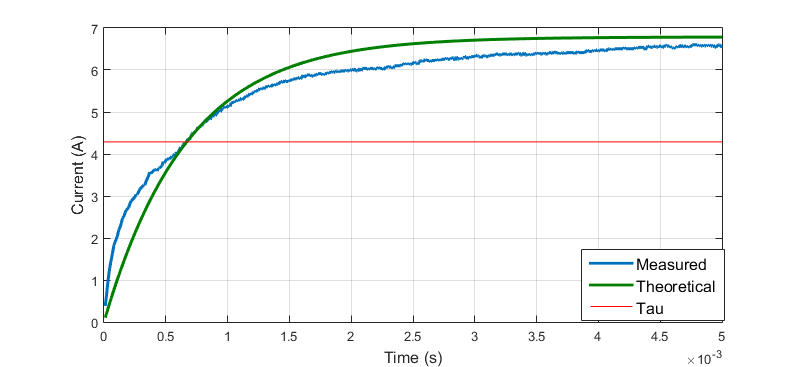
\includegraphics[width=1\textwidth]{figures/motor2ndExersize}
	\caption{Plot of test results}
\end{figure}

When the system is held in steady state, the inductor is a short circuit, which is the reason for the measure, while the system is in steady state. In steady state the equation will be $I_a (s) = \frac{U_a (s)}{R_a} \longrightarrow R_a = \frac{U_a (s)}{I_a (s)}.$ This will be a linear function. The slope of the fitted curve line is $0.178$, which give a resistor on $0.178 \Omega$.